\documentclass[10pt]{article}
\usepackage[utf8x]{inputenc}
\usepackage{amsmath,color}
\usepackage{geometry}
%\usepackage[mathcal]{euscript}
\geometry{ top=2.5cm, bottom=2cm, left=2cm, right=2cm}
%\usepackage[authoryear]{natbib}
% \usepackage{pdflscape}
%\geometry{papersize={216mm,330mm}, top=3cm, bottom=2.5cm, left=4cm,  right=2cm}
\usepackage{graphicx}
\usepackage{siunitx}
\usepackage{booktabs}

\newcommand{\D}{\partial}
\newcommand{\Diff}[2] {\dfrac{\partial( #1)}{\partial #2}}
\newcommand{\diff}[2] {\dfrac{\partial #1}{\partial #2}}
\newcommand{\bv}[1]{\ensuremath{\mbox{\boldmath$ #1 $}}}
\newcommand{\gv}[1]{\ensuremath{\mbox{\boldmath$ #1 $}}}% for vectors of Greek letters
\newcommand{\grad}[1]{\gv{\nabla} #1}
\newcommand{\Rho}{\,\mathtt{Rho}}
\newcommand{\PP}{\,\mathtt{P}}
\newcommand{\U}{\,\mathtt{U}}
\newcommand{\V}{\,\mathtt{V}}
\newcommand{\W}{\,\mathtt{W}}
\newcommand{\Lo}{\,\mathcal{L}}
\newcommand{\convection}{\,\text{convection}}
\newcommand{\production}{\,\text{production}}
\newcommand{\diffusion}{\,\text{diffusion}}
\newcommand{\gradp}{\,\text{grad}p}
\newcommand{\dissipation}{\,\text{dissipation}}
\newcommand{\todo}[1]{ {\color{blue} #1} }
%opening
\title{Manufactured Solution for the 3D Incompressible Navier-Stokes equation}
\author{Kemelli C. Estacio-Hiroms, Rhys Ulerich, Nick Malaya, Robert Moser}

\begin{document}



	
\maketitle
% 
% \begin{abstract}
% The Method of Manufactured Solutions is a valuable approach for code verification, providing means to verify how accurately the numerical method solves the partial differential equations of interest.
% This document presents the source terms generated by the application of the Method of Manufactured Solutions (MMS) for an incompressible turbulence flow  using the analytical manufactured solutions for velocity presented by \cite{Rhys2011}.
% \end{abstract}





\section{Mathematical model}
The governing equations for a incompressible flow can be written as:% \cite{Kim1987}:
\begin{equation}
 \label{eq:ns_01}
\diff{\bv{u}}{t}  = -\nabla p +\bv{H} +  \nu \nabla^2 \bv{u},
\end{equation}
\begin{equation}
 \label{eq:ns_02}
\nabla \cdot \bv{u} = 0.
\end{equation}


% Here, all the variables are non-dimensionalized by the channel half-width $\delta$, and the wall shear velocity $u_\tau$. $\bv{u}=(u,v,w)$, $\bv{H}=\bv{u}\cdot\nabla\bv{u}$ and $Re$ denotes the Reynolds number defined as $Re=u_\tau  \delta / \nu$.


Here, $\bv{u}=(u,v,w)$,  $\nu$ denotes the viscosity (constant) and $\bv{H}=-\bv{u}\cdot\nabla\bv{u}$, ie,
\begin{eqnarray}
 H_1 = - \left(\diff{ u^2}{x}+\diff{ uv }{y} +\diff{ uw}{z} \right)\\
 H_2 = - \left(\diff{ uv }{x}+\diff{ v^2}{y} +\diff{ vw}{z} \right)\\
 H_3 = - \left(\diff{ uw }{x}+\diff{ vw }{y} +\diff{ w^2}{z} \right).
\end{eqnarray}

The boundary conditions of the channel flow are:
$$u=v=w =0 \quad \mbox{at} \quad y=\pm 1.$$

The pressure can be calculated by solving the following Poisson equation:
\begin{equation}
\label{eq:ns_03}
\nabla \cdot \bv{H} = \nabla^2 p 
\end{equation}
when the nonlinear terms are calculated. Eq.~(\ref{eq:ns_03}) is obtained by taking the derivatives of each component of Eq.~ (\ref{eq:ns_01}) and summing all directions.

\section{Manufactured solution}

The Method of Manufactured Solutions (MMS) applied to the incompressible Navier--Stokes equations consists in modifying Equations~(\ref{eq:ns_01}) by adding a source term to the right-hand side of each equation, so the modified set of equations conveniently has the analytical solution chosen \textit{a priori}.

For the channel-flow case, it is necessary that the manufactured solutions satisfy a few important criteria:
\begin{itemize}
\item the analytical manufactured solutions must be periodic in $x$ and $z$ directions;
\item the analytical manufactured solutions must be finite in $y$ with no-slip on two boundary $xz$ planes (e.g. $y=0$ and $y=Ly$).
\item the analytical manufactured solutions must be sufficiently complex in the interior of the channel, i.e., they must have non-vanishing, time-varying mixed partial derivatives on $u$, $v$, and $w$ up to second order.
\item they should satisfy the incompressibility condition imposed by Equation (\ref{eq:ns_02}).
\end{itemize}

Even though there is no equation for the pressure in the incompressible Navier-Stokes equations, two of the above requirements is also true to the manufactured solutions for pressure $p$: it must be sufficiently complex in the channel as to exercises all the terms involving $p$ in the equations; and it must be periodic in $x$ and $z$ directions, but not in the $y$-direction. 


%There are two different sets of manufactured solutions chosen for verifying the Incompressible Navier-Stokes.

%The first set is:
Choosing the manufactured solutions to be of the form:
\begin{equation}
\begin{split}\label{eq:uvw01}
u(x,y,z,t)&= \alpha \sin\left( \frac{k_l x}{L_x} + \frac{a_{12}t}{L_t} \right) \cos\left( \frac{k_n z}{L_z} + \frac{b_{12}t}{L_t} \right) g'(y)\\
v(x,y,z,t)&=        \cos\left( \frac{k_l x}{L_x} + \frac{a_{12}t}{L_t} \right) \cos\left( \frac{k_n z}{L_z} + \frac{b_{12}t}{L_t} \right) g(y)\\ 
w(x,y,z,t)&=  \beta \cos\left( \frac{k_l x}{L_x} + \frac{a_{12}t}{L_t} \right) \sin\left( \frac{k_n z}{L_z} + \frac{b_{12}t}{L_t} \right) g'(y)\\
p(x,y,z,t)&=  \cos\left( \frac{k_l x}{L_x} + \frac{a_{12}t}{L_t} \right) \sin\left( \frac{k_n z}{L_z} + \frac{b_{12}t}{L_t} \right) \\
\end{split}
\end{equation}
with
%If we choose
\begin{equation}\label{eq:ab01}
\alpha = -\dfrac{k_l}{k_l^2+ k_n^2}\quad\mbox{and}\quad \beta = -\dfrac{k_n}{k_l^2+ k_n^2} 
\end{equation}
then the incompressibility restriction imposed by the continuity equation is satisfied. In order to ensure that mixed derivatives are not zero, one must choose $g=g(y)$ such as $g''(y) \neq 0$.

% 
% The second set of equations is:
% \begin{equation}
% \begin{split}\label{eq:uvw02}
% u(x,y,z,t)&= \alpha \sin\left( k_l x + a_{12}t \right) \cos\left( k_n z + b_{12}t \right) h(y)\\
% v(x,y,z,t)&= 0\\
% w(x,y,z,t)&=  \beta \cos\left( k_l x + a_{12}t \right) \sin\left( k_n z + b_{12}t \right) h(y)\\
% \end{split}
% \end{equation}
% And, in this case, choosing
% \begin{equation}
% \alpha = -k_n \quad\mbox{and}\quad \beta = -k_l 
% \end{equation}
% guarantees incompressibility.

%By construction, 
In order to the manufactured solutions for $u$, $v$ and $w$ satisfy the boundary conditions, it is sufficient that both function $g$ and its derivative $g'$ satisfy the boundary conditions, i.e.: $g(y)=0$ and $g'(y)=0$ at $y=0$ and $y=Ly$. A few choices of functions $g$ that satisfy these requirements are:
\begin{align}
\label{eq:g1}
g &= \dfrac{L_y^2}{\pi} \cos\left(\dfrac{\pi y}{L_y}\right)+y^2-\dfrac{L_y^2}{4} , \quad \mbox{or}\\
\label{eq:g2}
g &= \dfrac{L_y^2}{\pi} \cos\left(\dfrac{\pi y}{L_y}\right)+y^2-\dfrac{L_y^2}{4} +y^2 \left(y-\dfrac{L_y}{2} \right)^2 \left(y+\dfrac{L_y}{2} \right)^2, \quad \mbox{or}\\
\label{eq:g3}
g &= \dfrac{L_y^2}{\pi} \cos\left(\dfrac{\pi y}{L_y}\right)+y^2-\dfrac{L_y^2}{4} +y^4 \left(y-\dfrac{L_y}{2} \right)^4 \left(y+\dfrac{L_y}{2} \right)^4, \quad \mbox{or}\\
\label{eq:g4}
g &= \dfrac{L_y^2}{\pi} \cos\left(\dfrac{\pi y}{L_y}\right)+y^2-\dfrac{L_y^2}{4} +y^4  \left(y-\dfrac{L_y}{2} \right)^2\left(y+\dfrac{L_y}{2} \right)^2, \quad \mbox{or}\\
\label{eq:g5}
g &= \dfrac{L_y^2}{\pi} \cos\left(\dfrac{\pi y}{L_y}\right)+y^2-\dfrac{L_y^2}{4} +y^2 \left(y-\dfrac{L_y}{2} \right)^4 \left(y+\dfrac{L_y}{2} \right)^4.
\end{align}



\subsection{The Method of Manufactured Solutions}


The MMS consists in modifying the incompressible Navier-Stokes equations~(\ref{eq:ns_01}) by adding a source term to the right-hand side of each equation:
\begin{equation}
\begin{split}\label{eq:ns_mod_2d}
&\diff{u}{t}  + \diff{p}{x} -H_1 -  \nu\left(\diff{^2 u}{ x^2}+\diff{^2 u}{ y^2}+\diff{^2 u}{ z^2} \right)=Q_u\\
&\diff{v}{t}  + \diff{p}{y} -H_2 -  \nu\left(\diff{^2 v}{ x^2}+\diff{^2 v}{ y^2}+\diff{^2 v}{ z^2} \right)=Q_v\\
&\diff{w}{t}  + \diff{p}{x} -H_3 -  \nu\left(\diff{^2 w}{ x^2}+\diff{^2 w}{ y^2}+\diff{^2 w}{ z^2} \right)=Q_w\\
\end{split}
\end{equation}
so the modified set of equations (\ref{eq:ns_mod_2d}) conveniently has the analytical solution given in Equations (\ref{eq:uvw01}), (\ref{eq:ab01}), and one choice for function $g$, given in Eqs. (\ref{eq:g1})--(\ref{eq:g5}).


\subsection{Choosing $g$}
We attempt to make the manufactured solution to resemble the inner portion (viscous sublayer + logarithmic
layer) of a zero pressure gradient boundary layer. For that, we follow Pope's description of the Reynolds stress of a turbulent flow in a channel~\cite{pope2000turbulent}, and try to reproduce such behavior with the proposed manufactured solutions.

The boundary condition $u=v=w=0$ at the wall determines the way in which the Reynolds stresses depart from zero for small $y$. For fixed $x$, $z$ and $t$, and for small $y$, the fluctuating velocity components can be written as Taylor series of the form:
\begin{equation}
\begin{split}
u &= a_1 + b_1 y + c_1 y^2 + \dots, \\
v &= a_2 + b_2 y + c_2 y^2 + \dots, \\
w &= a_3 + b_3 y + c_3 y^2 + \dots, \\ 
\end{split}
\end{equation}

The coefficients are zero-mean random variable, and, for fully developed channel flow, they are statistically independent of $x$, $z$ and $t$. For $y=0$, the no-slip condition yields $u=a_1=0$ and $w=a_3=0$; and the impermeability condition yields $v=a_2=0$. At the wall, since $u$ and $v$ are zero for all $x$ and $z$,  the derivatives $(\partial u/ \partial x)|_{y=0}$ and $(\partial w/ \partial z)|_{y=0}$ are also zero; hence the continuity equation yiels v$(\partial v/ \partial y)|_{y=0}=b_2=0$.
\todo{actually, our wall is at y=+-1. So I am not sure how this will work. Rhys\&Nick, I need your input here.}

The Reynolds stresses can be obtained from the expansions above simply by taking means of the products of the series. Taking account of the coefficients that are zero ($a_1$, $a_2$, $a_3$ and $b_2$), the leading order in $y$ of the Reynolds stresses are:
\begin{equation}
\begin{split}
\langle u^2 \rangle &= \langle b_1^2 \rangle y^2  + \dots, \\
\langle v^2 \rangle &= \langle c_2^2 \rangle y^4 + \dots, \\
\langle uv  \rangle &= \langle b_1 c_2 \rangle y^2 + \dots, \\
\langle w^2 \rangle &= \langle b_3^2 \rangle y^3 + \dots, 
\end{split}
\end{equation}
Thus, while $\langle u^2 \rangle$ and $\langle w^2 \rangle$ increase from zero as $y^2$, $\langle uv  \rangle$ and 
$\langle w^2 \rangle$ increase more slowly, as $y^3$ and $y^4$, respectively. Therefore, we seek for manufactured solutions that mostly closely reproduce such behavior.


Recall that the instantaneous velocity $u'$ can be written as the sum of the fluctuating velocity $u$ with the average velocity $\langle u\rangle$, i.e:
$$u'=u+\langle u\rangle$$

The Reynolds stresses can be obtained from the manufactured solutions by taking the mean (expectation) of the fluctuating velocity squared:
\begin{equation}
\begin{split}\label{eq:exp_Reynolds}
\langle u^2\rangle &= \langle (u'-\langle u\rangle)^2 \rangle = \langle{u'}^2\rangle - \langle u\rangle^2 \\
\langle v^2\rangle &= \langle {v'}^2 \rangle - \langle v\rangle^2 \\ 
\langle w^2\rangle &= \langle {w'}^2 \rangle- \langle w\rangle^2 \\
\langle uv \rangle &= \langle u'v' \rangle - \langle u\rangle\langle v\rangle \\  
\end{split}
\end{equation}
where the average (expectation) of a function $u$ is defined by:
\begin{equation}\label{eq:expectation}
\langle u \rangle = E[[u(x,y,z,t)]]\big\rvert_{xzt}= \dfrac{1}{t_f L_x L_z} \int_{t=0}^{t_f} \int_{-L_x/2}^{L_x/2} \int_{-L_z/2}^{L_z/2} u(x,y,z,t) \;dz\,dx\,dt  
\end{equation}


In order to calculate the Reynolds stress (through averaging fluctuating velocities), one must select parameters for both the manufactured solution, Eq. (\ref{eq:ns_mod_2d}), and chosen $g$ function, Eq. (\ref{eq:g1})--(\ref{eq:g5}). A convenient set of parameters is given in Table \ref{table:parameters}. Note that with these choices the manufactured solution satisfies no-slip conditions at $y = -L_y/2$ and $y=L_y/2$.
\begin{table}[htpb]
\caption{Parameter recommendations.}
\vspace{-8pt}
\begin{center}
\begin{tabular}{cc|cc|cc}
\toprule
Constant & Value & Constant & Value & Constant & Value \\
\midrule\midrule
$L_x$	& $4\pi$ & $L_t$  	& 1      & $k_n$ 	& 11 \\
$L_y$	& 2      & $t_f$  	& 5      & $a_{12}$ & 7  \\
$L_z$ 	& $3\pi$ & $k_l$ 	& 5      & $b_{12}$ & 13 \\[0.4ex]
\bottomrule
\end{tabular}
\end{center}
\label{table:parameters}
\end{table}

Using the parameters presented in Table \ref{table:parameters}, it is possible to calculate the expectations of the terms in Equation~(\ref{eq:exp_Reynolds}) using the definition given in Equation (\ref{eq:expectation}). The formula for $\langle u^2 \rangle$ and its Taylor expansion is given in  Table~\ref{table:exp_u}, for each function $g$ presented in Equations (\ref{eq:g1})--(\ref{eq:g5}). The Taylor expansion for the remaining terms ($\langle uv \rangle$, $\langle v^2 \rangle$ and $\langle w^2 \rangle$) is presented in Table \ref{table:taylor}. All the calculations are carried out using MAPLE.

Analyzing the data presented in Tables \ref{table:exp_u} and \ref{table:taylor}, we conclude that the behavior mostly closely related to the one described by Pope~\cite{pope2000turbulent} is achieved when the function $g$ is given by Equation XXX. \todo{$\longleftarrow$ Nick/Rhys, this is with you :)}

\begin{table}[htpb]
\caption{Expectation of $u^2$ ($\langle u^2 \rangle$) and its approximation with Taylor series.}
\vspace{-8pt}
\begin{center}
\begin{tabular}{c|c|c}
\toprule
$g$ & $\langle u^2 \rangle$ & Taylor series   \\
\midrule\midrule
Eq. (\ref{eq:g1}) &$0.1857338391 \sin(\pi y / 2)^2-0.3714676782 \sin(\pi y / 2) y+0.1857338391 y^2$	& $0.06051365368 y^2+O(y^4)$\\
Eq. (\ref{eq:g2}) &$0.04643345978 (-2 \sin(\pi y / 2)+4 y+6 y^5-8 y^3)^2$	& $0.03421510645 y^2+O(y^4)$\\
Eq. (\ref{eq:g3}) &$0.04643345978 (-2 \sin(\pi y / 2)+2 y+48 y^7-24 y^5+4 y^3+12 y^11-40 y^9)^2$& $0.06051365368 y^2+O(y^4)$ \\
Eq. (\ref{eq:g4}) &$0.04643345978 (-2 \sin(\pi y / 2)+2 y+8 y^7-12 y^5+4 y^3)^2$	& $0.06051365368 y^2+O(y^4)$\\
Eq. (\ref{eq:g5}) &$0.04643345978 (-2 \sin(\pi y / 2)+4 y+36 y^5-16 y^3+10 y^9-32 y^7)^2$	& $0.03421510645 y^2+O(y^4)$\\
\bottomrule
\end{tabular}
\end{center}
\label{table:exp_u}
\end{table}

\begin{table}[htpb]
\caption{Taylor series of expectation of $v^2$, $uv$ and $w^2$.}
\vspace{-8pt}
\begin{center}
\scriptsize
\begin{tabular}{c|c|c|c}
\toprule
$g$ & $\langle v^2 \rangle$ &  $\langle uv \rangle$ & $\langle w^2 \rangle$  \\
\midrule\midrule
Eq. (\ref{eq:g1}) &$0.01863596445-0.07786091193 y^2+O(y^4)$&$-0.00004251718738 y+0.0001369344824 y^3+O(y^5)$&$0.1638380546 y^2+O(y^4)$\\
Eq. (\ref{eq:g2}) &$0.01863596445+0.05854660928 y^2+O(y^4)$&$0.00003197030557 y-0.0001996148868 y^3+O(y^5)$&$0.09263589518 y^2+O(y^4)$\\
Eq. (\ref{eq:g3}) &$0.01863596445-0.07786091193 y^2+O(y^4)$&$-0.00004251718738 y+0.0002859094683 y^3+O(y^5)$&$0.1638380546 y^2+O(y^4)$\\
Eq. (\ref{eq:g4}) &$0.01863596445-0.07786091193 y^2+O(y^4)$&$-0.00004251718738 y+0.0002859094683 y^3+O(y^5)$&$0.1638380546 y^2+O(y^4)$\\
Eq. (\ref{eq:g5}) &$0.01863596445+0.05854660928 y^2+O(y^4)$&$0.00003197030557 y-0.0004975648584 y^3+O(y^5)$&$0.09263589518 y^2+O(y^4)$\\
\bottomrule
\end{tabular}
\end{center}
\label{table:taylor}
\end{table}


\begin{figure}[thb]
\centering
%\includegraphics[width=0.495\textwidth]{channel-geometry}
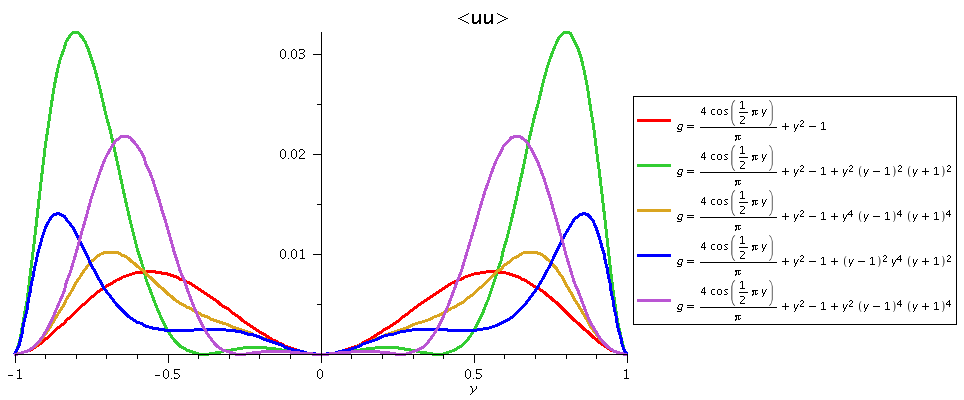
\includegraphics[scale=0.35]{uu.png}
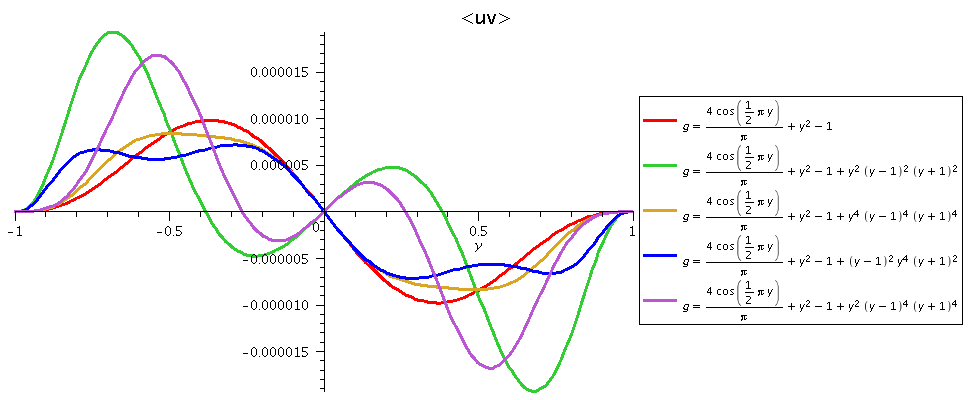
\includegraphics[scale=0.35]{uv.png}
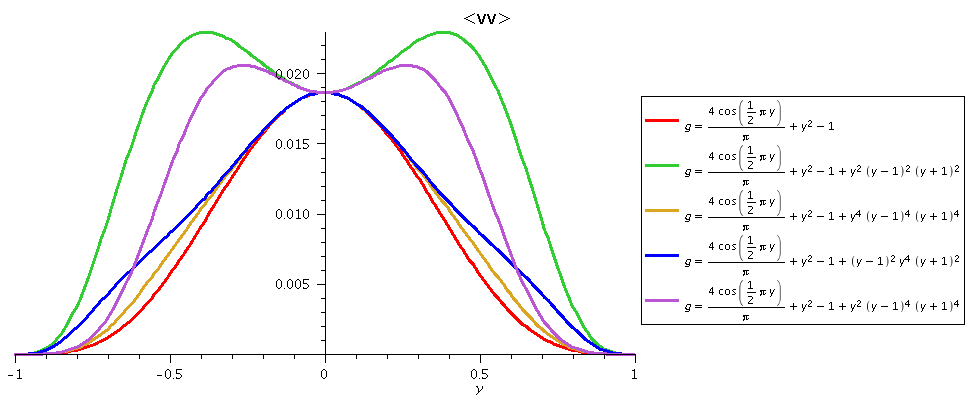
\includegraphics[scale=0.35]{vv.png}
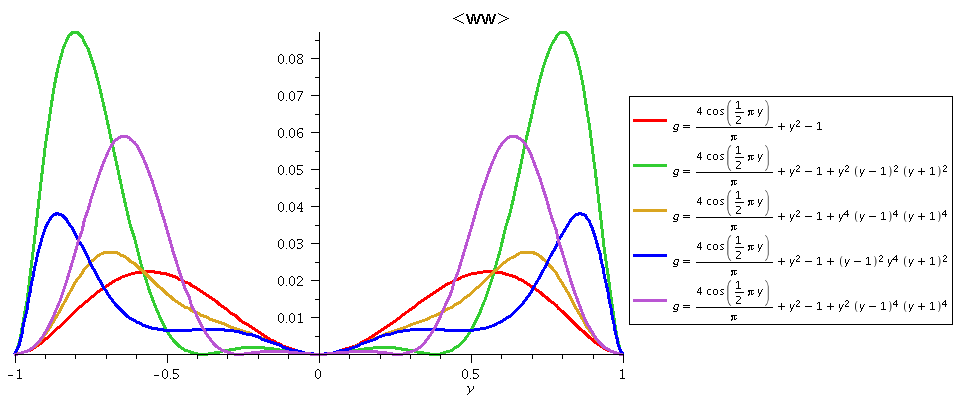
\includegraphics[scale=0.35]{ww.png}
  \\[-0.2cm]
  \caption{Expectations of $u^2$, $v^2$, $uv$ and $w^2$.
           \label{fig:expectations}}
\end{figure}



% 
% Thus, we use Equations (\ref{eq:uvw01}), (\ref{eq:ab01}), (\ref{eq:g}) and (\ref{eq:p}) and the Method of Manufactured Solutions to obtain source terms $Q_u$, $Q_v$ and $Q_w$, in such way that modified by the inclusion of such source terms:
% \begin{equation}
% \begin{split}
% &\diff{u}{t}  + \diff{p}{x} -H_1 -  \nu\left(\diff{^2 u}{ x^2}+\diff{^2 u}{ y^2}+\diff{^2 u}{ z^2} \right)=Q_u\\
% &\diff{v}{t}  + \diff{p}{y} -H_2 -  \nu\left(\diff{^2 v}{ x^2}+\diff{^2 v}{ y^2}+\diff{^2 v}{ z^2} \right)=Q_v\\
% &\diff{w}{t}  + \diff{p}{x} -H_3 -  \nu\left(\diff{^2 w}{ x^2}+\diff{^2 w}{ y^2}+\diff{^2 w}{ z^2} \right)=Q_w\\
% \end{split}
% \end{equation}
% have known, analytical solutions given, in turn, by Equation (\ref{eq:uvw01}) -- which satisfies the incompressibility condition:
% \begin{equation*}
% \diff{u}{x}+\diff{v}{y}+\diff{w}{z}= 0.
% \end{equation*}


 \begin{thebibliography}{99}

\bibitem{pope2000turbulent}
S. B. Pope. Turbulent Flows, Cambridge University Press, 2000.

 \end{thebibliography}

\end{document}

\subsection{Streamwise velocity}

% For the generation of the analytical source term $Q_u$ for the $x$-momentum equation, Equation  (\ref{eq:euler_02}) is written as an  operator $\Lo$:
% \begin{equation*}
%  \Lo=\diff{u}{t}  + \diff{p}{x} -H_1 -  \nu\left(\diff{^2 u}{ x^2}+\diff{^2 u}{ y^2}+\diff{^2 u}{ z^2} \right)
% \end{equation*}

For the generation of the analytical source term $Q_u$, $x$-momentum equation (\ref{eq:ns_01}) is written as an operator $\Lo_u$:
 $$\Lo_u = \Lo_{u \, \text{time}}+\Lo_{u \, \convection}+\Lo_{u \, \gradp }+\Lo_{u \, \dissipation }$$
with each one of the sub-operators defined as follows:

\begin{equation}
 \begin{split}
\Lo_{u \, \text{time}}&= \diff{u}{t}  \\
\Lo_{u \, \convection}&= -H_1\\
\Lo_{u \, \gradp }&= \Diff{p}{x}\\
\Lo_{u \, \dissipation }&= - \nu\left(\diff{^2 u}{ x^2}+\diff{^2 u}{ y^2}+\diff{^2 u}{ z^2} \right)
 \end{split}
\end{equation}
%
which, when operated in Equation (\ref{eq:uvw01}),  (\ref{eq:g}) and~(\ref{eq:p}), provides source term $Q_{u}$:
\begin{equation*} 
Q_u = Q_{u \, \text{time}}+Q_{u \, \convection}+Q_{u \, \gradp }+Q_{u \, \dissipation }
\end{equation*}
where:
\begin{equation*}
\begin{split}
Q_{u \,\text{time}} &=-\left(-a_{12} \cos\left(a_{12} t+k_l x\right) \cos\left(b_{12} t+k_n z\right)+b_{12} \sin\left(a_{12} t+k_l x\right) \sin\left(b_{12} t+k_n z\right)\right) \alpha \frac{dg}{dy}\\
%
 Q_{u \convection} &= -\alpha \, g''(y) \, \cos\left(a_{12} t+k_l x\right) \cos\left(b_{12} t+k_n z\right)^2 g \sin\left(a_{12} t+k_l x\right)+\\
	&- \left(\alpha k_l \cos\left(b_{12} t+k_n z\right)^2-\beta k_n \sin\left(b_{12} t+k_n z\right)^2\right) \alpha \, g'(y)^2 \cos\left(a_{12} t+k_l x\right) \sin\left(a_{12} t+k_l x\right) \\
%
Q_{u \gradp} &=\alpha \, g''(y) \, \cos\left(a_{12} t+k_l x\right) \cos\left(b_{12} t+k_n z\right)^2 g \sin\left(a_{12} t+k_l x\right)+\\
	&+\left(\alpha k_l \cos\left(b_{12} t+k_n z\right)^2-\beta k_n \sin\left(b_{12} t+k_n z\right)^2\right) \alpha \, g'(y)^2 \cos\left(a_{12} t+k_l x\right) \sin\left(a_{12} t+k_l x\right) \\
%
 Q_{u \dissipation} &=-\alpha\, g'''(y) \, \nu \cos\left(b_{12} t+k_n z\right) \sin\left(a_{12} t+k_l x\right)+\left(k_l^2+k_n^2\right) \alpha \, g'(y) \,\nu \cos\left(b_{12} t+k_n z\right) \sin\left(a_{12} t+k_l x\right)\\\vspace{8pt}
\end{split}
\end{equation*}
%
where $g$ is given in Equation (\ref{eq:g}) and its derivatives are:
\begin{equation}
\begin{split}\label{eq:derivative_g}
\, g'(y) \,&= \dfrac{L_y^4 y}{2}-\dfrac{9 L_y^3 y^2}{2} +13 L_y^2 y^3-15 L_y y^4+6 y^5+L_y \cos\left(\dfrac{\pi y}{L_y}\right)-L_y+2 y\\
%
\, g''(y) \, &=  \dfrac{L_y^4}{2}-9 L_y^3 y+39 L_y^2 y^2-60 L_y y^3+30 y^4-\pi \sin\left(\dfrac{\pi y}{L_y}\right)+2\\
%
\, g'''(y) \,  &= -9 L_y^3+78 L_y^2 y-180 L_y y^2+120 y^3-\dfrac{\pi^2}{L_y} \cos\left(\dfrac{\pi y}{L_y}\right)
\end{split}
\end{equation}

\subsection{Wall-normal velocity}
For the generation of the analytical source term $Q_v$, $y$-momentum equation (\ref{eq:ns_01}) is written as an operator $\Lo_v$:
 $$\Lo_v = \Lo_{v \, \text{time}}+\Lo_{v \, \convection}+\Lo_{v \, \gradp }+\Lo_{v \, \dissipation }$$
with each one of the sub-operators defined as follows:

\begin{equation}
 \begin{split}
\Lo_{v \, \text{time}}&= \diff{v}{t}  \\
\Lo_{v \, \convection}&= -H_2\\
\Lo_{v \, \gradp }&= \Diff{p}{y}\\
\Lo_{v \, \dissipation }&= - \nu\left(\diff{^2 v}{ x^2}+\diff{^2 v}{ y^2}+\diff{^2 v}{ z^2} \right)
 \end{split}
\end{equation}
%
which, when operated in Equation (\ref{eq:uvw01}),  (\ref{eq:g}) and~(\ref{eq:p}), provides source term $Q_{v}$:
\begin{equation*} 
Q_v = Q_{v \, \text{time}}+Q_{v \, \convection}+Q_{v \, \gradp }+Q_{v \, \dissipation }
\end{equation*}
where:
\begin{equation*}
\begin{split}
Q_{v \,\text{time}} &=-\left(a_{12} \cos\left(b_{12} t+k_n z\right) \sin\left(a_{12} t+k_l x\right)+b_{12} \cos\left(a_{12} t+k_l x\right) \sin\left(b_{12} t+k_n z\right)\right) \, g\\
%
 Q_{v \convection} &= \left(\alpha k_l \cos\left(b_{12} t+k_n z\right)^2 \sin\left(a_{12} t+k_l x\right)^2+\beta k_n \cos\left(a_{12} t+k_l x\right)^2 \sin\left(b_{12} t+k_n z\right)^2 +\right.\\
	&\left.-\cos\left(a_{12} t+k_l x\right)^2 \cos\left(b_{12} t+k_n z\right)^2\right) \, g'(y) \,\, g\\
%
Q_{v \gradp} &= \left(-\alpha k_l \cos\left(b_{12} t+k_n z\right)^2 \sin\left(a_{12} t+k_l x\right)^2-\beta k_n \cos\left(a_{12} t+k_l x\right)^2 \sin\left(b_{12} t+k_n z\right)^2+\right.\\
	&\left.+\cos\left(a_{12} t+k_l x\right)^2 \cos\left(b_{12} t+k_n z\right)^2\right) \, g'(y) \,\, g\\
%
 Q_{v \dissipation} &=\left(-\frac{d^2g}{dy^2}+\left(k_l^2+k_n^2\right) \, g\right) \nu \cos\left(a_{12} t+k_l x\right) \cos\left(b_{12} t+k_n z\right)\\\vspace{8pt}
\end{split}
\end{equation*}
where $g$ is given in Equation (\ref{eq:g}) and its derivatives are given in Equation (\ref{eq:derivative_g}).

\subsection{Spanwise velocity}
For the generation of the analytical source term $Q_w$, $z$-momentum equation (\ref{eq:ns_01}) is written as an operator $\Lo_w$:
 $$\Lo_w = \Lo_{w \, \text{time}}+\Lo_{w \, \convection}+\Lo_{w \, \gradp }+\Lo_{w \, \dissipation }$$
with each one of the sub-operators defined as follows:

\begin{equation}
 \begin{split}
\Lo_{w \, \text{time}}&= \diff{w}{t}  \\
\Lo_{w \, \convection}&= -H_3\\
\Lo_{w \, \gradp }&= \Diff{p}{z}\\
\Lo_{w \, \dissipation }&= - \nu\left(\diff{^2 w}{ x^2}+\diff{^2 w}{ y^2}+\diff{^2 w}{ z^2} \right)
 \end{split}
\end{equation}
%
which, when operated in Equation (\ref{eq:uvw01}),  (\ref{eq:g}) and~(\ref{eq:p}), provides source term $Q_{w}$:
\begin{equation*} 
Q_w = Q_{w \, \text{time}}+Q_{w \, \convection}+Q_{w \, \gradp }+Q_{w \, \dissipation }
\end{equation*}
where:
\begin{equation*}
\begin{split}
Q_{w \,\text{time}} &=-\left(a_{12} \sin\left(a_{12} t+k_l x\right) \sin\left(b_{12} t+k_n z\right)-b_{12} \cos\left(a_{12} t+k_l x\right) \cos\left(b_{12} t+k_n z\right)\right) \beta \frac{dg}{dy}\\
%
 Q_{w \convection} &= -\beta \, g''(y) \, \cos\left(a_{12} t+k_l x\right)^2 \cos\left(b_{12} t+k_n z\right) \, g \sin\left(b_{12} t+k_n z\right)+ \\
	&+\left(\alpha k_l \sin\left(a_{12} t+k_l x\right)^2-\beta k_n \cos\left(a_{12} t+k_l x\right)^2\right) \beta \, g'(y)^2 \cos\left(b_{12} t+k_n z\right) \sin\left(b_{12} t+k_n z\right)\\
%
Q_{w \gradp} &=\beta \, g''(y) \, \cos\left(a_{12} t+k_l x\right)^2 \cos\left(b_{12} t+k_n z\right) \, g \sin\left(b_{12} t+k_n z\right)+ \\
	&-\left(\alpha k_l \sin\left(a_{12} t+k_l x\right)^2-\beta k_n \cos\left(a_{12} t+k_l x\right)^2\right) \beta \, g'(y)^2 \cos\left(b_{12} t+k_n z\right) \sin\left(b_{12} t+k_n z\right)\\
%
 Q_{w \dissipation} &=\left(-\dfrac{d^3g}{dy^3}+\left(k_l^2+k_n^2\right) \frac{dg}{dy}\right) \beta \nu \cos\left(a_{12} t+k_l x\right) \sin\left(b_{12} t+k_n z\right)\\\vspace{8pt}
\end{split}
\end{equation*}
where $g$ is given in Equation (\ref{eq:g}) and its derivatives are given in Equation (\ref{eq:derivative_g}).

% %---------------------------------------------------------------------------------------------------------

% 
 \begin{thebibliography}{99}
%  \bibitem{Ulerich2012}
% R.~Ulerich, {K.~C. Estacio-Hiroms}, N.~Malaya, R.~D. Moser, ``A Transient Manufactured Solution For The Compressible Navier-Stokes Equations with a Power Law Viscosity''. {\it 10th World Congress on Computational Mechanics}, S\~ao Paulo-Brazil, 8-12 July 2012.\\  
% 
\bibitem{pope2000turbulent}
S. B. Pope. Turbulent Flows, Cambridge University Press, 2000.
}

% \end{thebibliography}


\end{document}

